\subsection{Performance from Fingerprint images\label{fp-performance}}

The performance from the fingerprint images acquired from each of the fingers in shown in Fig. \ref{fingerprint-performance}. A commercial fingerprint matcher is used for the fingerprint matching as it offered the best performance (more details in Section \ref{discussion}) among the three fingerprint matchers considered in this work. It can be observed from the ROC curves in these images that, unlike for respective finger knuckle, the fingerprint images from the thumbs (thumbprints) offer the best performance. This is followed by the performance from the middle fingers. The thumbs are expected to generate superior performance and this can be attributed to the relative convenience during such imaging as the users find it easy to firmly press thumbs during the 4-4-2 fingerprint imaging. 

\begin{figure}[ht]
    \centering
    \subfloat[]{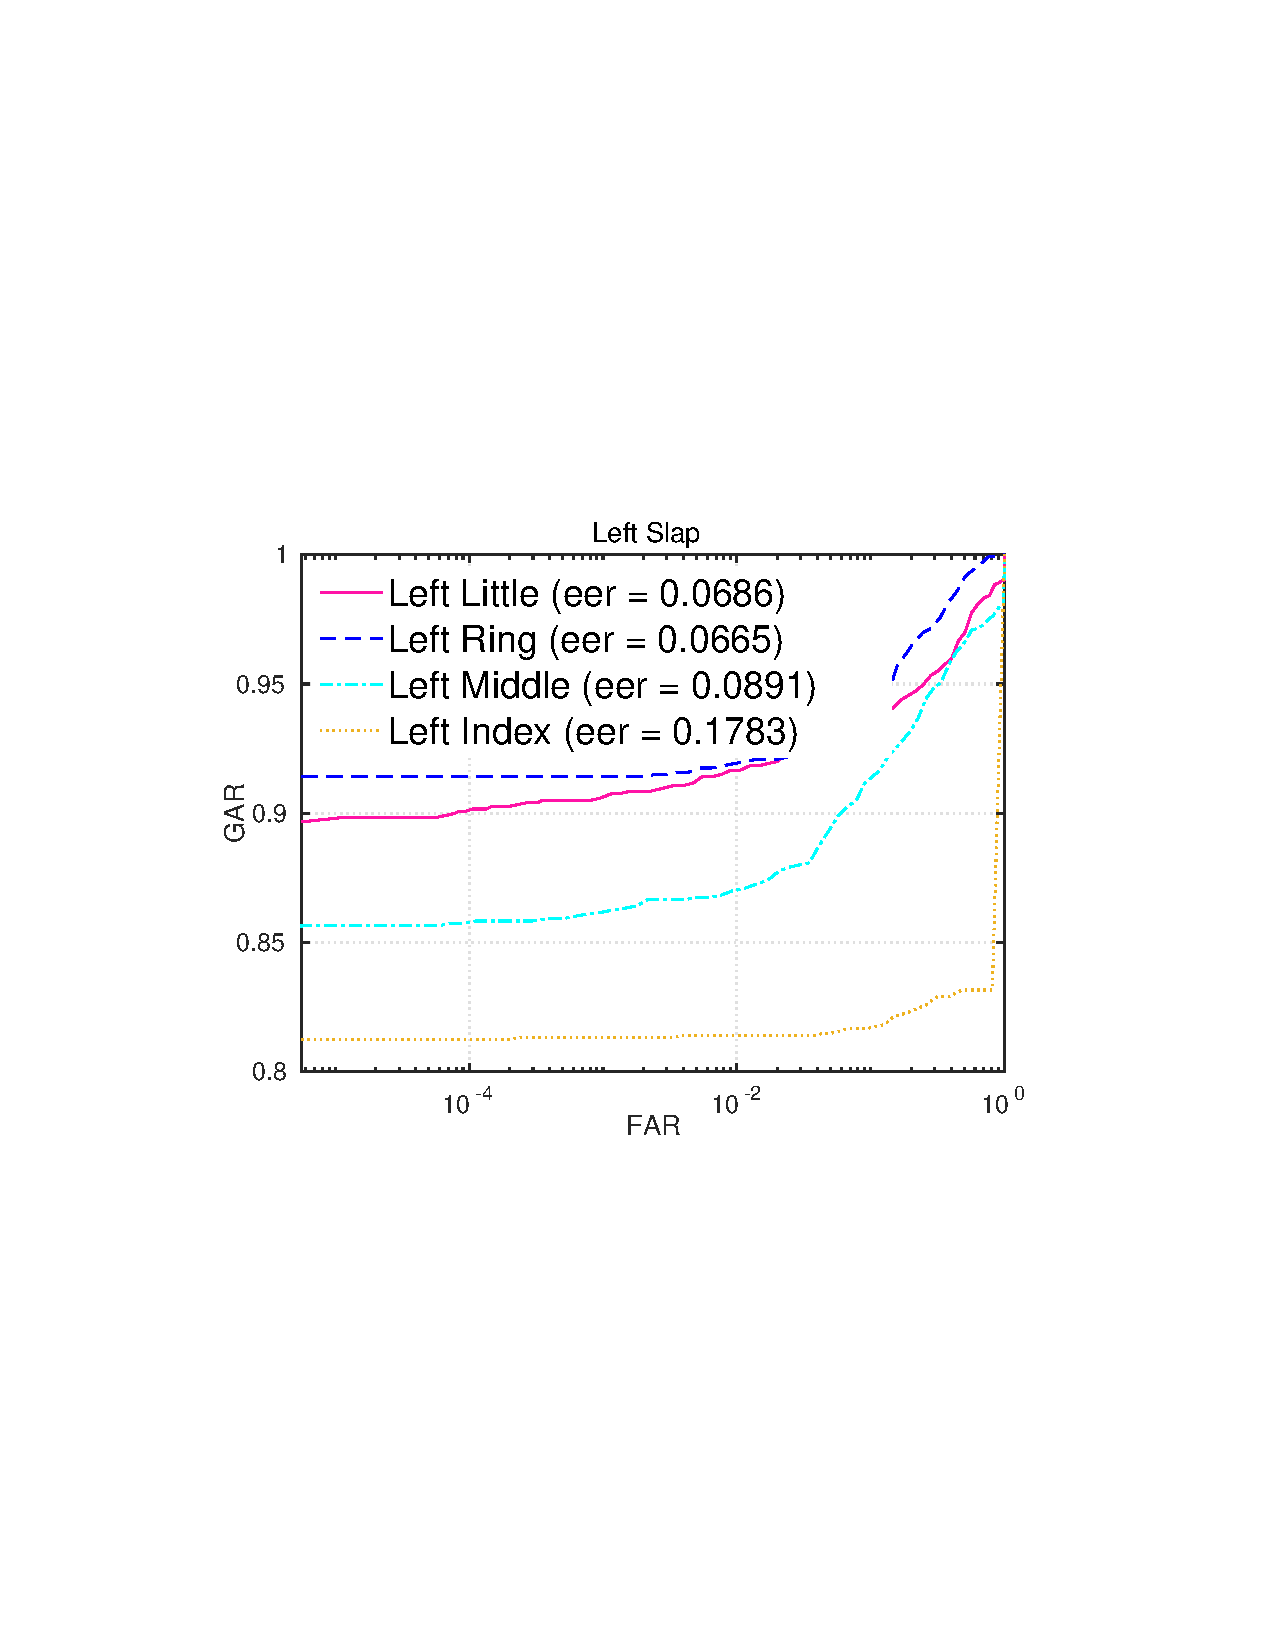
\includegraphics[width=1.7in]{Figures/fingerprint/left-roc.pdf}
    \label{}}
    \subfloat[]{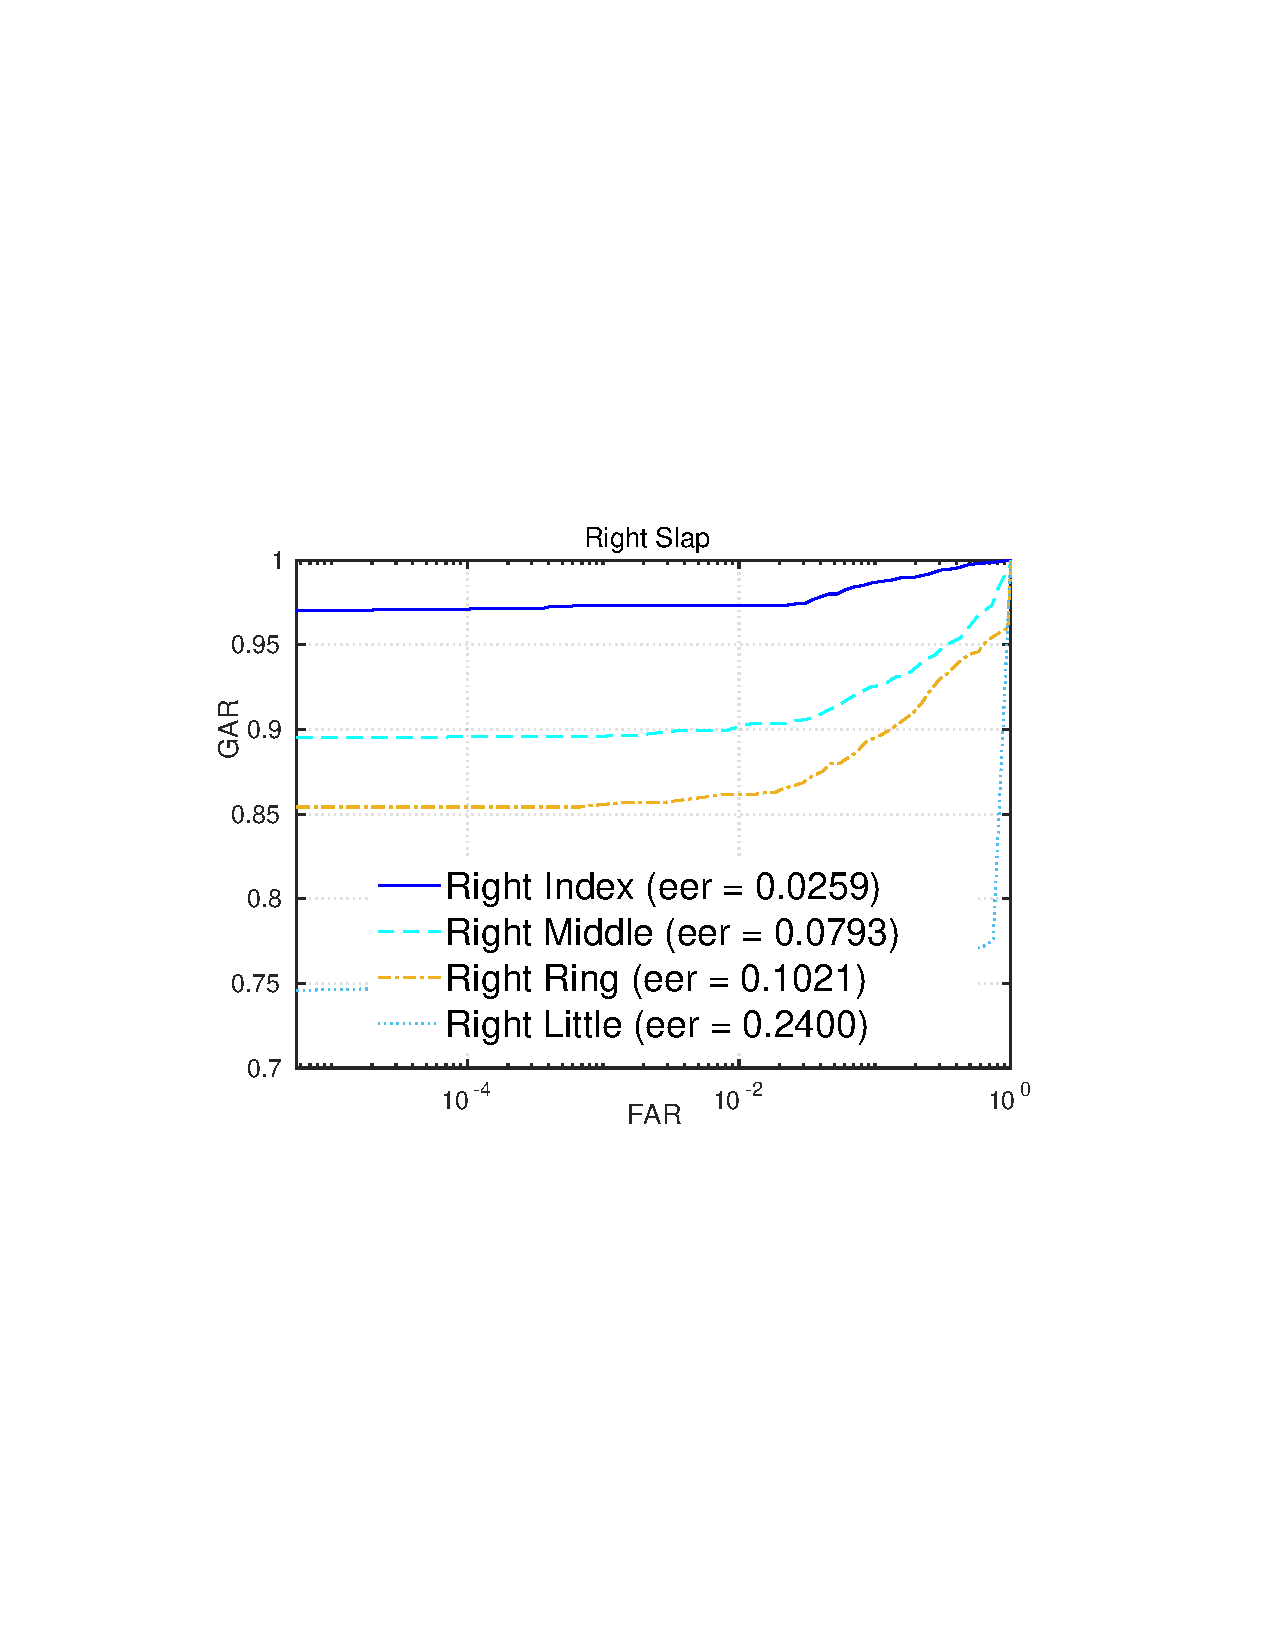
\includegraphics[width=1.75in]{Figures/fingerprint/right-roc.pdf}
    \label{}}

    \subfloat[]{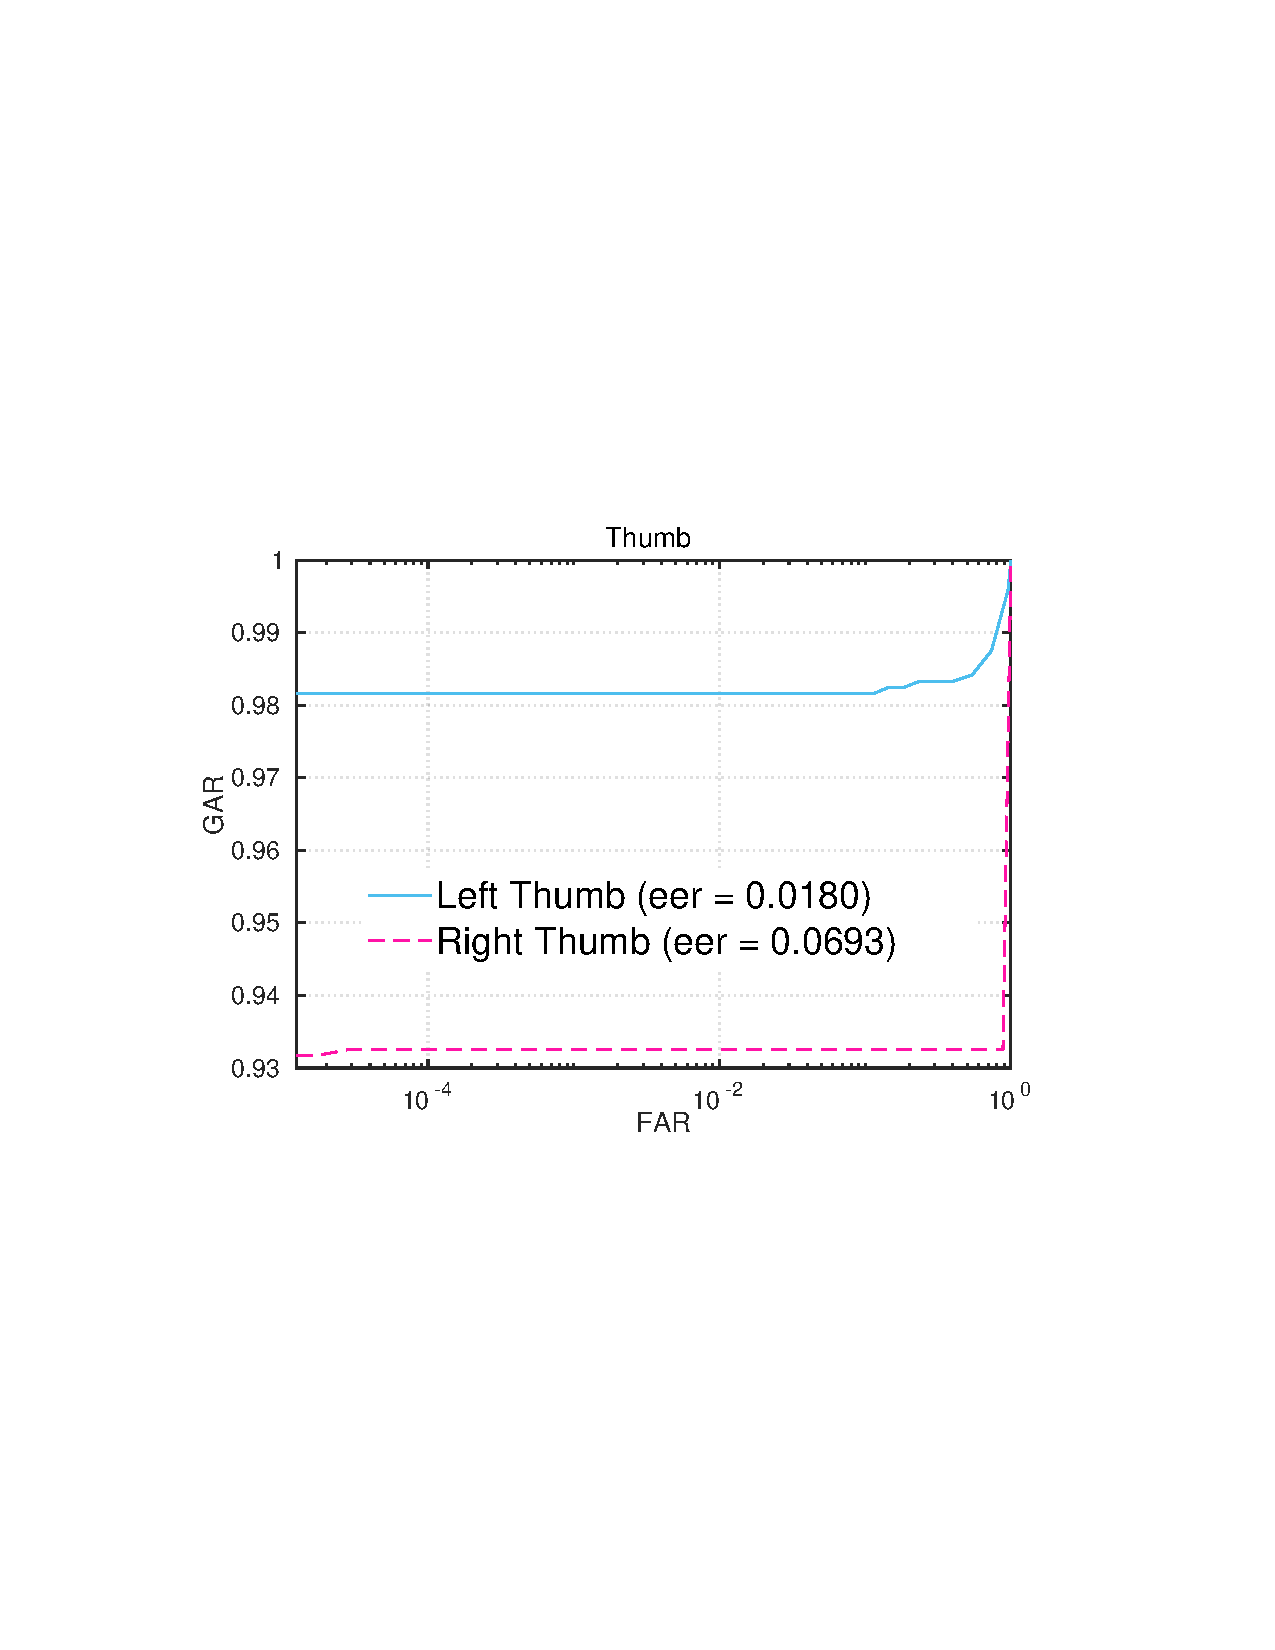
\includegraphics[width=1.8in]{Figures/fingerprint/thumb-roc.pdf}
    \label{}}
    \caption{Performance from the fingerprint images acquired using a slap-fingerprint sensor for (a) left hand, (b) right hand, and (c) thumbs under 4-4-2 imaging protocols.}
    \label{fingerprint-performance}
\end{figure}